\documentclass{article}

\usepackage[a4paper, total={6in, 8in}]{geometry}
\usepackage{setspace}

\usepackage[czech]{babel}
\usepackage[utf8]{inputenc}
\usepackage[T1]{fontenc}

\usepackage{amsmath,amsfonts,amssymb,amsthm,mathtools}
\usepackage{graphicx, subcaption}

\usepackage{hyperref}
\hypersetup{
	colorlinks,
	citecolor=blue,
	filecolor=black,
	linkcolor=blue,
	urlcolor=blue
}

\def\({\left(}
\def\){\right)}
\def\endl{\\[3mm]}

\renewcommand{\vec}{\boldsymbol}
\renewcommand{\d}{\mathrm d}
\newcommand{\e}{\mathrm e}
\newcommand{\h}{\hbar}

\onehalfspacing

\begin{document}
	\pagenumbering{gobble}
	
	\begin{center}
		\section*{Figure template document}
		\noindent\rule{15cm}{1.4pt}
	\end{center}
	
	\begin{figure}[h!]
		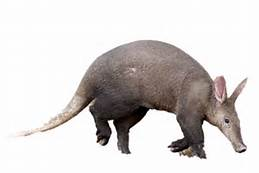
\includegraphics[width=\linewidth]{images/frajer.jpeg}
		\caption{Frajeros}
		\label{fig:frajer}
	\end{figure}
	
	Ty brďo to je \ref{fig:frajer} jak Kalousek.
	
	\subsection*{Image positioning}
		\begin{itemize}
			\item h (here) - same location,
			
			\item t (top) - top of page,
			
			\item b (bottom) - bottom of page,
			
			\item p (page) - on an extra page,
			
			\item ! (override) - will force the specified location.
		\end{itemize}
	\newpage
	
	Subfigures dáváj vedle sebe víš jak.
	
	\begin{figure}[h!]
		\centering
		\begin{subfigure}[b]{0.4\linewidth}
			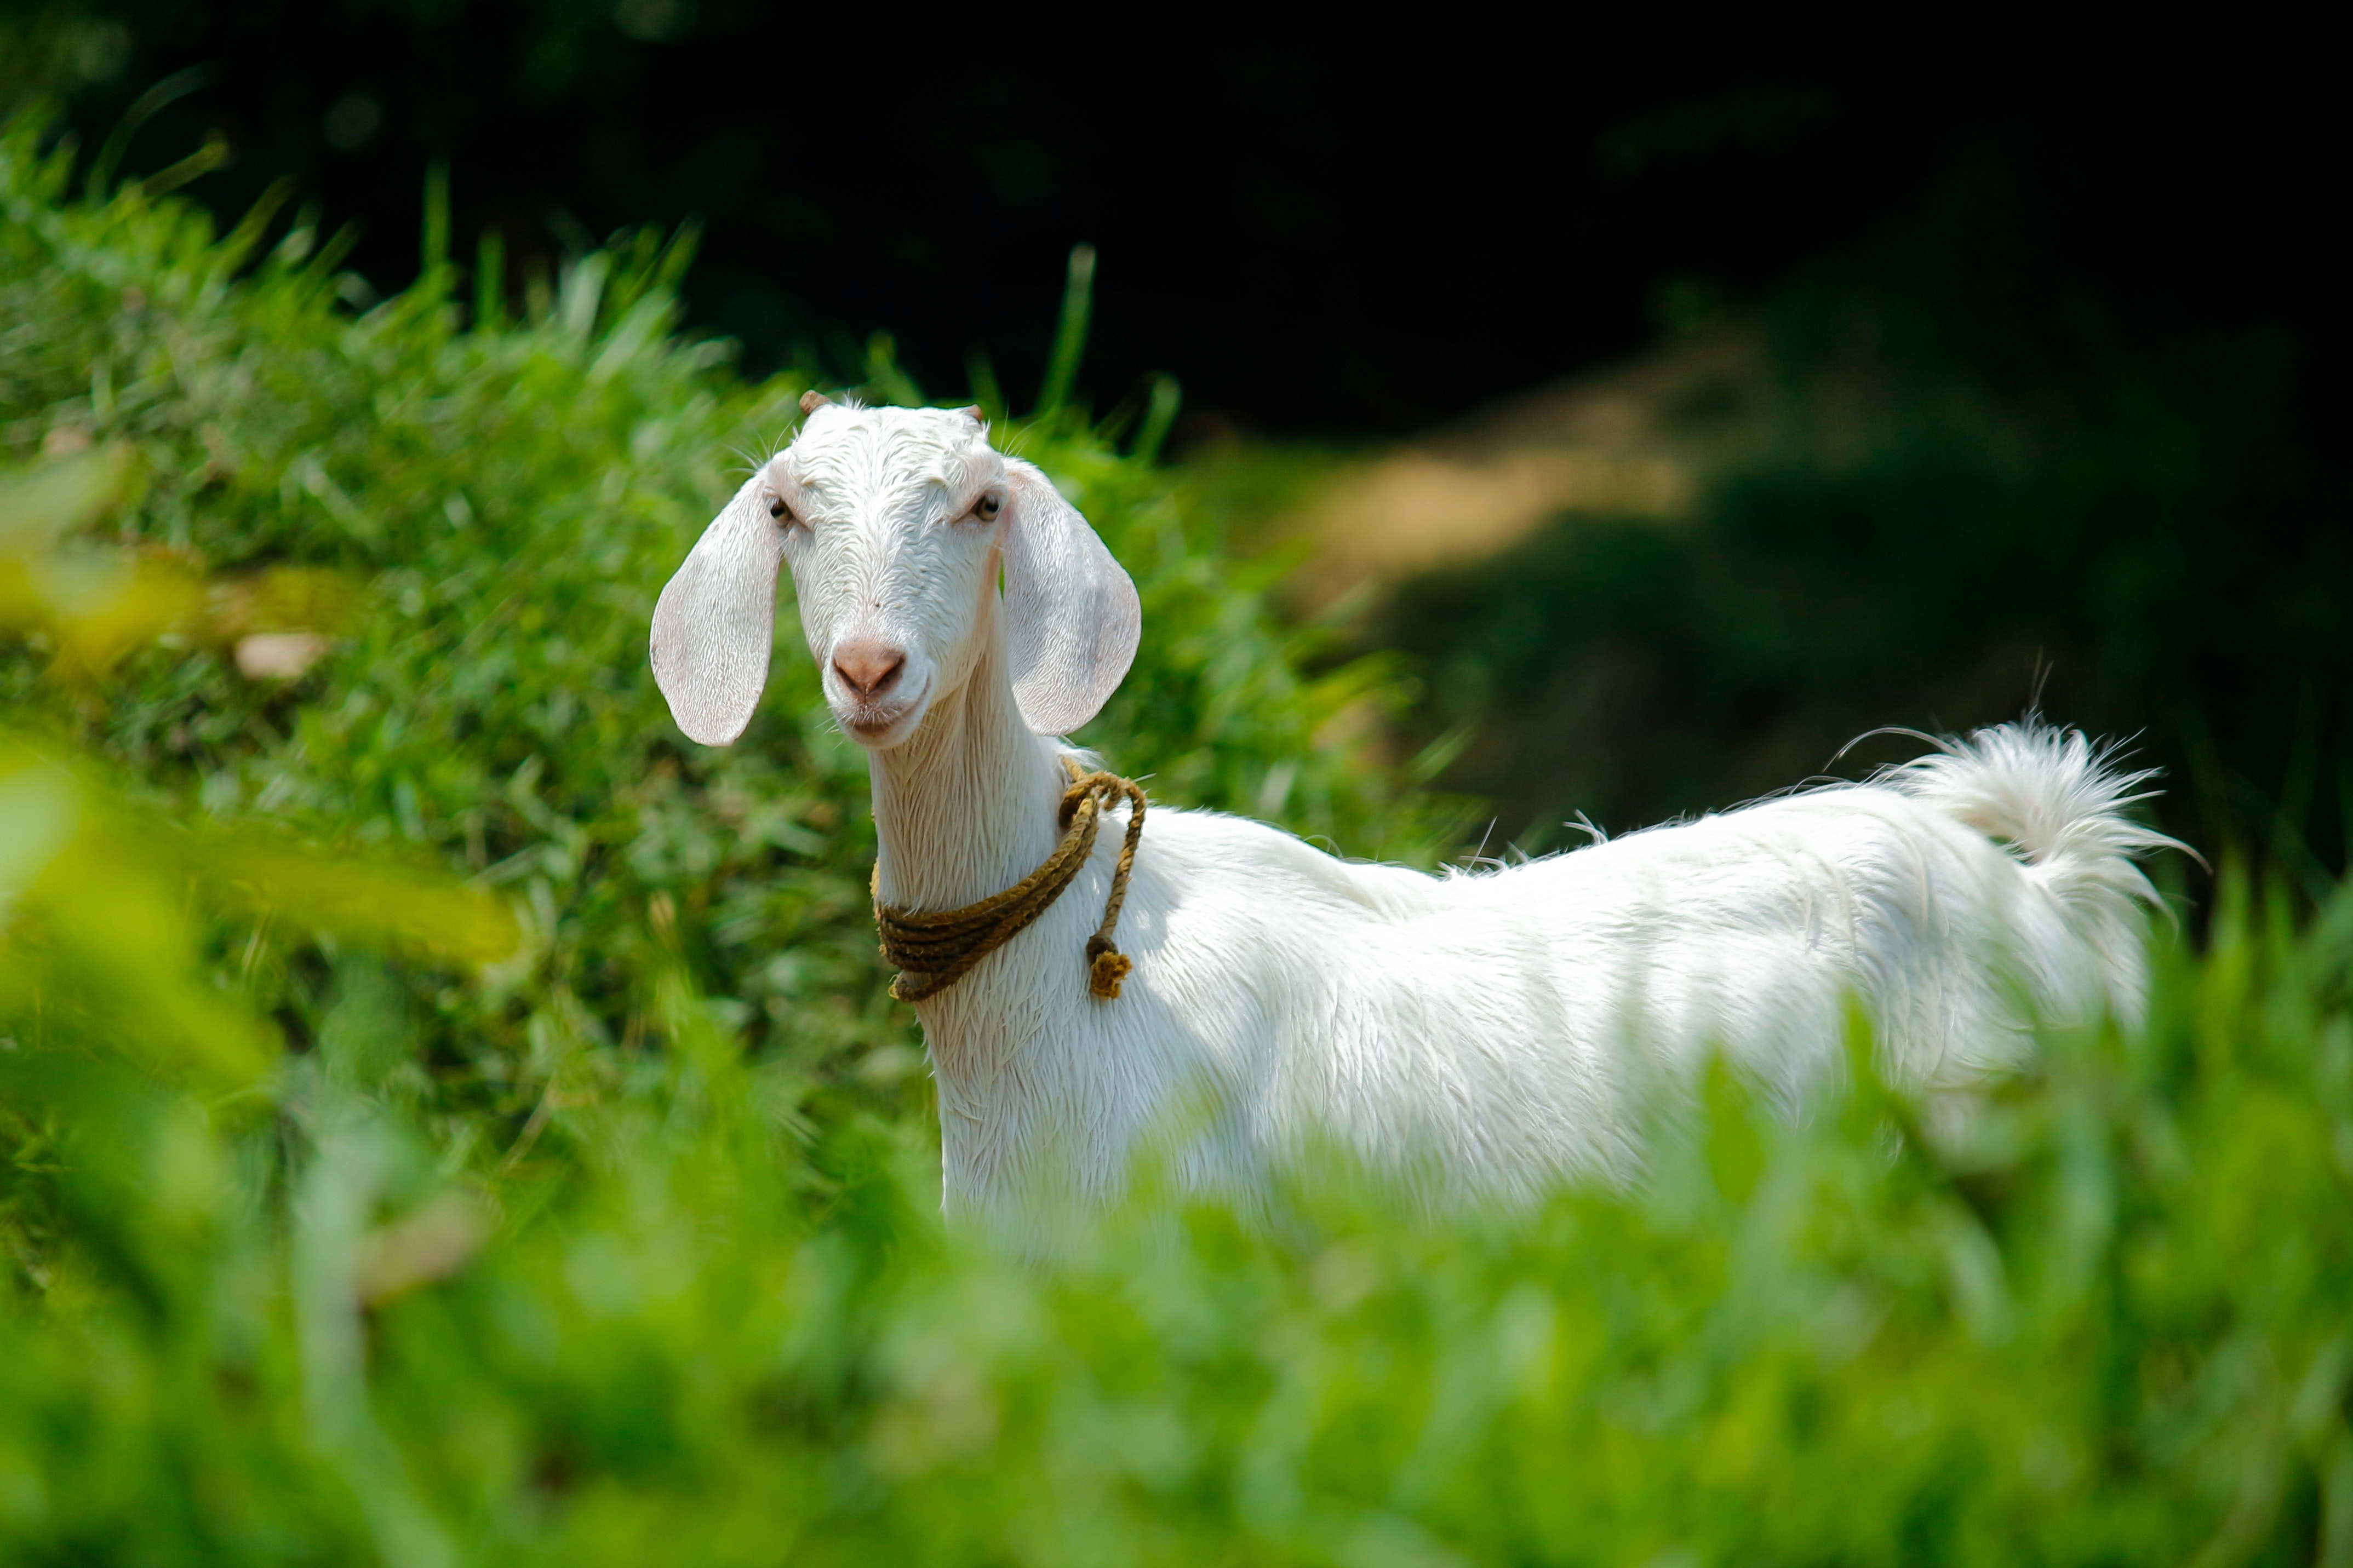
\includegraphics[width=\linewidth]{images/goat.jpg}
			\caption{A focken goat}
		\end{subfigure}
		\begin{subfigure}[b]{0.4\linewidth}
			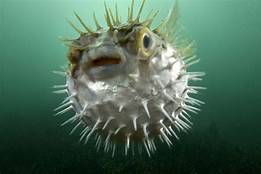
\includegraphics[width=\linewidth]{images/spikyboi.jpeg}
			\caption{Spikyboi}
		\end{subfigure}
		\caption{Two of the most dangerous bad bois you can encounter.}
		\label{fig:bois}
	\end{figure}
	Co teď? Checkuj frajera \ref{fig:frajer} eště jednou.
	
	\begin{figure}
		\centering
		\begin{subfigure}[b]{0.2\linewidth}
			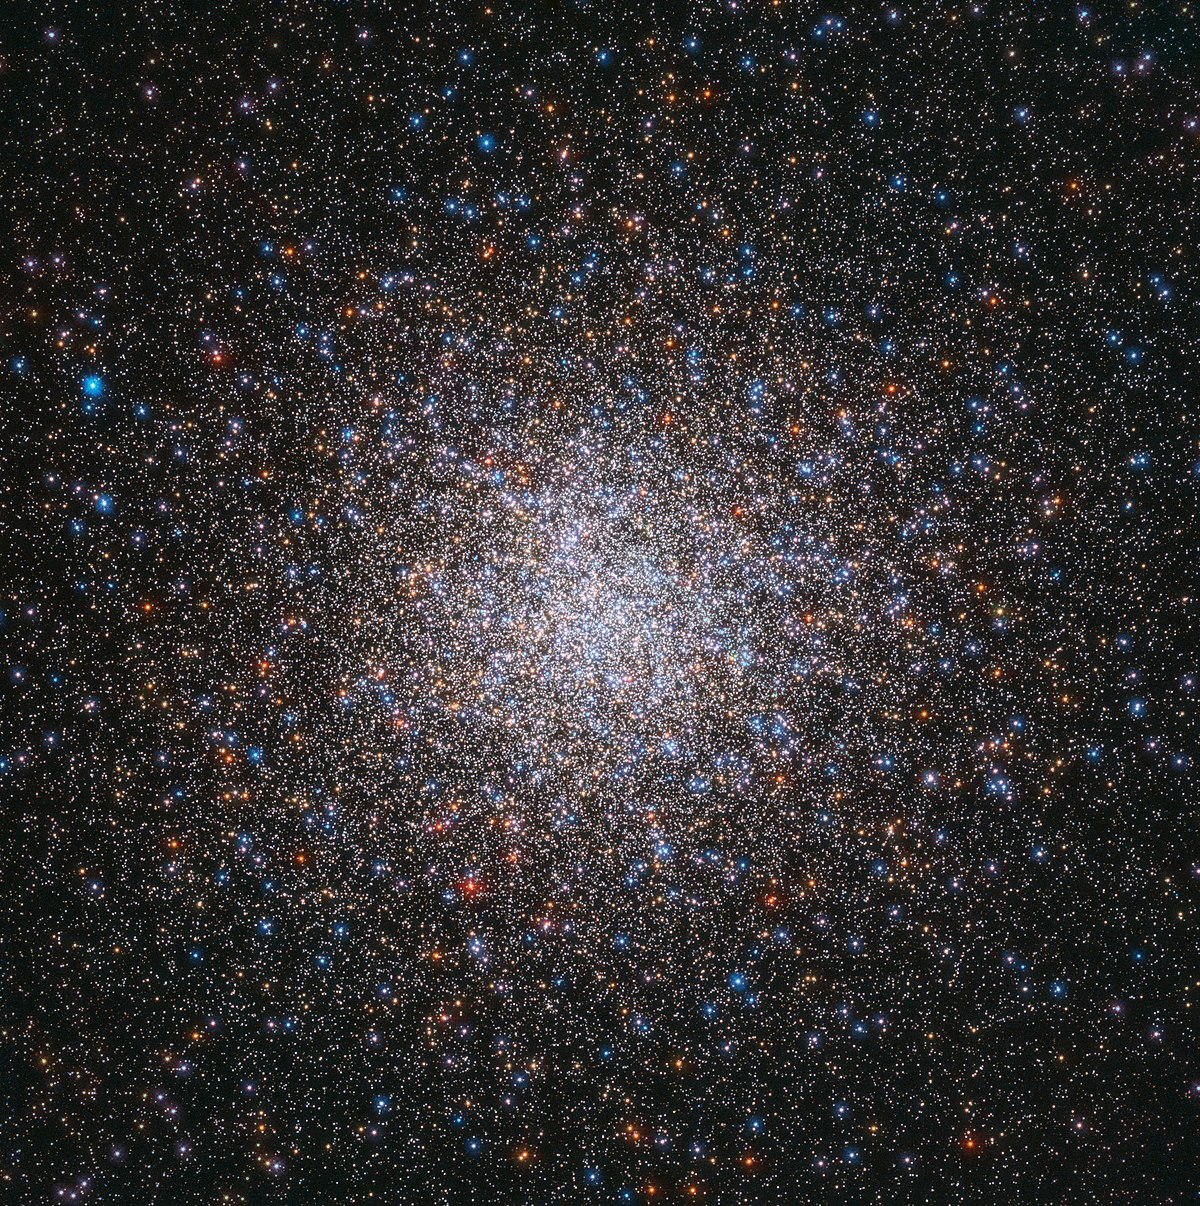
\includegraphics[width=\linewidth]{images/messier2.jpg}
			\caption{Messier 2}
		\end{subfigure}
		\begin{subfigure}[b]{0.2\linewidth}
			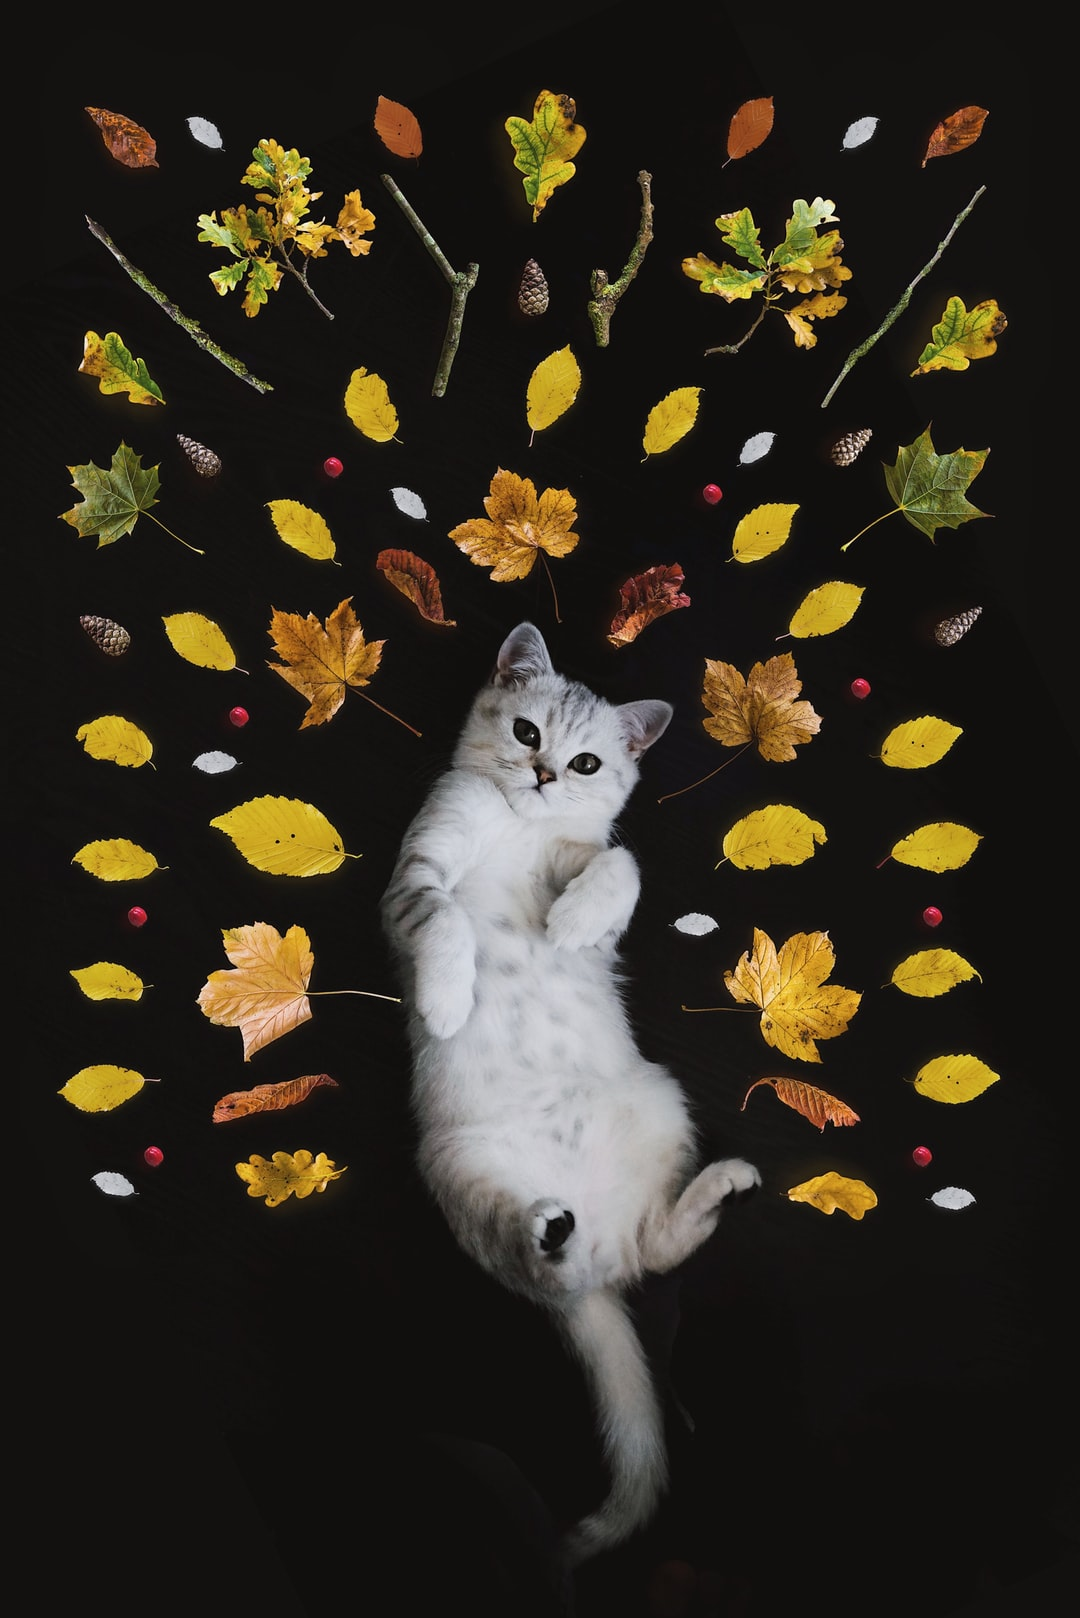
\includegraphics[width=\linewidth]{images/wtf.jpeg}
			\caption{Powerful cat aura}
		\end{subfigure}
		\begin{subfigure}[b]{0.2\linewidth}
			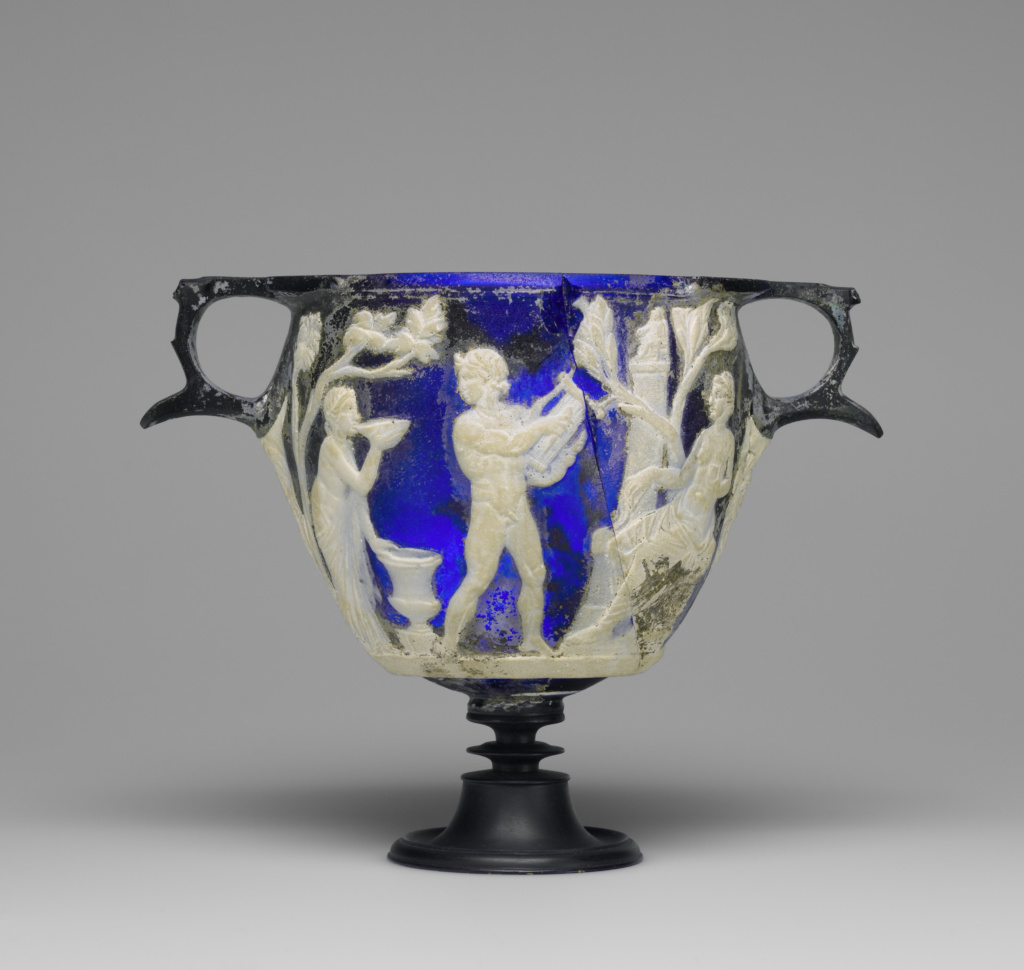
\includegraphics[width=\linewidth]{images/vase.jpg}
			\caption{An ancient vase}
		\end{subfigure}
		\begin{subfigure}[b]{0.5\linewidth}
			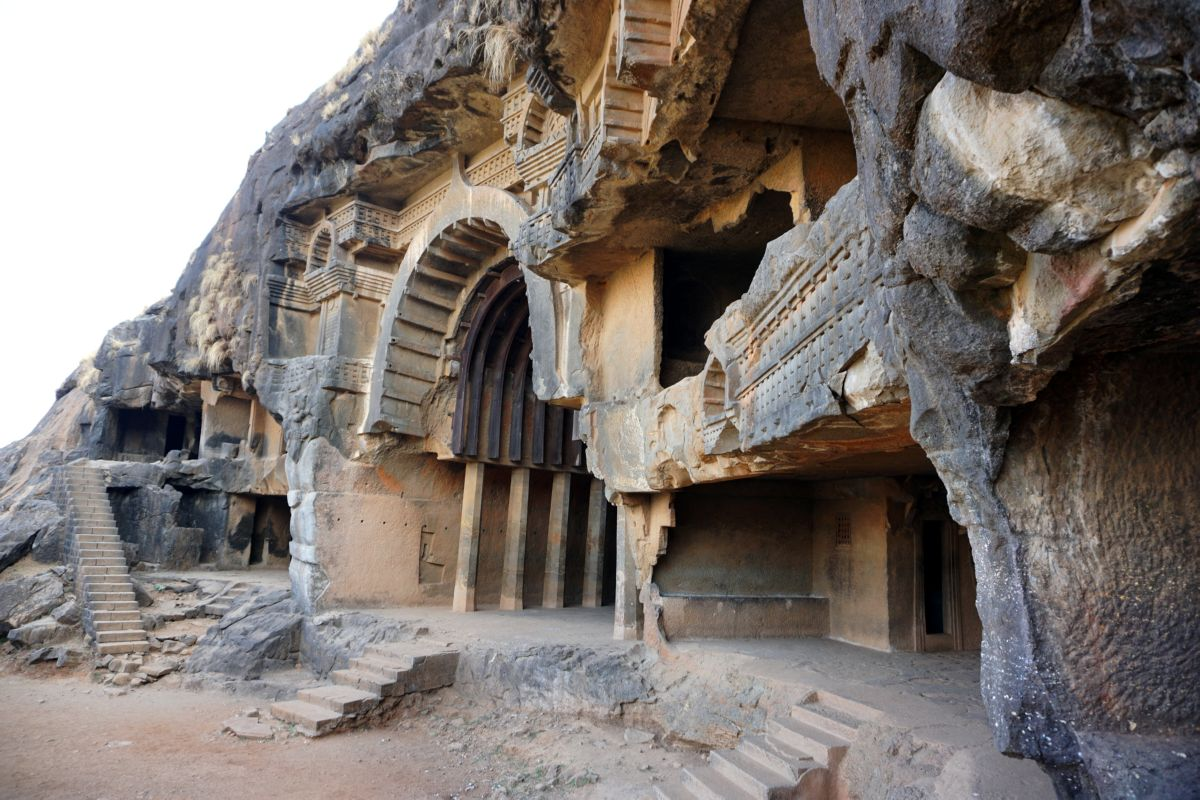
\includegraphics[width=\linewidth]{images/caves.jpg}
			\caption{Nice holes bby 8-)}
		\end{subfigure}
		\caption{Random mess}
		\label{fig:mess}
	\end{figure}
	\newpage
	
	\begin{appendix}
		\listoffigures
	\end{appendix}
	
	
\end{document}